\section{Comparaison avec les autres systèmes de stockage distribué}

Dans cette section, nous comparons brièvement Ceph avec les autres solutions de stockage distribué et expliquons les nouveautés apportées.

Nous ne traitons pas des systèmes de fichiers antiques ou peu utilisés, dont les inconvénients sont évidents\footnote{Mauvaise gestion de la réplication, existence systématique de SPOF\ldots} mais tentons de le comparer aux technologies plus modernes.

StorNext et EMC ScaleIO sont par exemple des solutions de stockage distribué propriétaires qui proposent une mise à l'échelle performantes, mais n'implémente pas de stockage unifié de niveau bloc, objet et système de fichiers.

GPFS permet d'atteindre d'excellentes performances, comprend la tolérance aux pannes et la redondance, mais n'est pas open-source. De plus, les systèmes similaires -- dits SAN pour Storage Area Network -- utilisent des \textit{disques durs en réseau}, et ne tirent absolument pas partie de l'intelligence collective. Ils comprennent en outre au moins un SPOF en le gestionnaire central qui coordonne l'accès aux disques.

D'autres solutions comme Lustre ou OpenZSF ont pris le parti de stocker les données en tant qu'objets plutôt qu'en tant que blocs. Ces objets intègrent en particulier les métadonnées propres aux données concernées. L'intelligence collective est alors possible. Pour autant, des systèmes comme Lustre ne délèguent que très peu de tâches aux composantes de stockage.

Gluster est une solution moderne très utilisée, mais ne propose pas de stockage unifié. Les performances de Ceph sont en général supérieures à celles de Gluster.

Swift, un des concurrents les plus sérieux de Ceph, ne propose pas non plus de stockage unifié. Ceph est plus performant, mais notons que le fonctionnement de Swift propose une sécurité supplémentaire. En effet, Ceph est sensible à la compromission d'une composante de stockage qui peut alors directement écouter tout le trafic non-chiffré. Swift, quant à lui, permet de séparer le réseau des \og{}clients\fg{} et celui des \og{}serveurs\fg{}.

La figure \ref{chap1:sec3:ceph_compare} résume la position de Ceph par rapport aux autres solutions. Elles ne sont pas toutes citées ici.

\begin{figure}
	\centering
    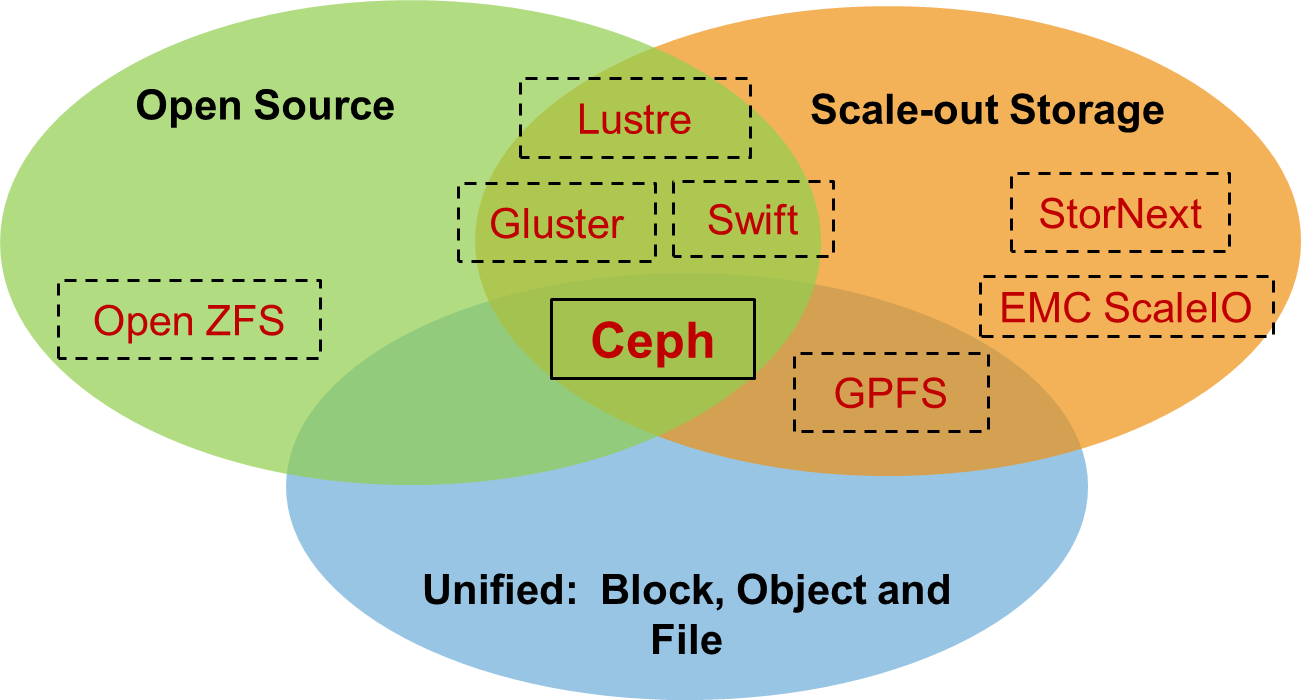
\includegraphics[scale=.5]{images/ceph_diagram.png}
    \caption{\label{chap1:sec3:ceph_compare}Comparaison de Ceph et des autres solutions de stockage distribué.}
\end{figure}

\begin{PimpedBox}
Ceph pourrait bien être une solution unique en offrant un ensemble de caractéristiques qu'aucune autre solution ne combine. Open-source, aisément évolutif, performant et extrêmement robuste, la sortie de la confidentialité du milieu universitaire pour être mis en production dans l'industrie témoigne de l'intérêt croissant pour Ceph.
\end{PimpedBox}